\subsubsection{monolith::component::widget::BaseWidgetView}

\label{monolith::component::widget::BaseWidgetView}
\begin{figure}[ht]
	\centering
	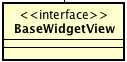
\includegraphics[scale=0.5]{Sezioni/SottosezioniST/img/BaseWidgetView.png}
	\caption{monolith::component::widget::BaseWidgetView}
\end{figure}

\begin{itemize}
\item \textbf{Descrizione:} Interfaccia che estende BaseComponent che rappresenta un qualsiasi widget che può essere inserito all'interno di un layout.
\item \textbf{Utilizzo:} Interfaccia che viene utilizzata ed implementata ogniqualvolta uno sviluppatore intende creare una nuova tipologia di widget che è possibile inserire all'interno di un layout.
\item \textbf{Attributi:}
\item \textbf{Metodi:}
\end{itemize}

\subsubsection{monolith::component::widget::button::ButtonWidgetView}

\label{monolith::component::widget::button::ButtonWidgetView}
\begin{figure}[ht]
	\centering
	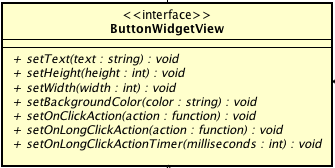
\includegraphics[scale=0.5]{Sezioni/SottosezioniST/img/ButtonWidgetView.png}
	\caption{monolith::component::widget::button::ButtonWidgetView}
\end{figure}

\begin{itemize}
\item \textbf{Descrizione}: Questa interfaccia rappresenta la view relativa ai widget di tipo bottone.
\item \textbf{Utilizzo}: L'interfaccia viene utilizzata per disaccoppiare presenter e implementazione del widget e per visualizzare i dati che gli vengono passati dal presenter.
\item \textbf{Attributi}:
\item \textbf{Metodi}:
	\begin{itemize}
	\item \textit{public setText(text:string):void}\\
	Imposta il testo all'interno del bottone.
		\\ \textbf{Parametri}: \begin{itemize}
		\item \textit{text:string}\\
		Rappresenta il testo che verrà impostato all'interno del bottone.
		\end{itemize}
	\item \textit{public setHeight(height:int):void}\\
	Imposta l'altezza del bottone.
		\\ \textbf{Parametri}: \begin{itemize}
		\item \textit{height:int}\\
		Rappresenta il numero di pixel corrispondente all'altezza del bottone che verrà impostata.
		\end{itemize}
	\item \textit{public setWidth(width:int):void}\\
	Imposta la larghezza del bottone.
		\\ \textbf{Parametri}: \begin{itemize}
		\item \textit{width:int}\\
		Rappresenta il numero di pixel corrispondente alla larghezza del bottone che verrà impostata.
		\end{itemize}
	\item \textit{public setBackgroundColor(color:string):void}\\
	Imposta il colore di sfondo del bottone.
		\\ \textbf{Parametri}: \begin{itemize}
		\item \textit{color:string}\\
		Rappresenta la stringa in esadecimale corrispondente al colore che verrà impostata come sfondo del bottone.
		\end{itemize}
	\item \textit{public setOnClickAction(action:function):void}\\
	Questo metodo viene utilizzato per impostare l'azione che deve essere eseguita dopo il click normale del bottone.
		\\ \textbf{Parametri}: \begin{itemize}
		\item \textit{action:function}\\
		L'azione, sotto forma di funzione, che deve essere eseguita al click normale del bottone.
		\end{itemize}
	\item \textit{public setOnLongClickAction(action:function):void}\\
		Questo metodo viene utilizzato per impostare l'azione che deve essere eseguita dopo il click prolungato del bottone.
		\\ \textbf{Parametri}: \begin{itemize}
		\item \textit{action:function}\\
		L'azione, sotto forma di funzione, che deve essere eseguita al click prolungato del bottone.
		\end{itemize}
		\item \textit{public setOnLongClickActionTimer(milliseconds:int):void}\\
		Questo metodo viene utilizzato per impostare il tempo che deve scorrere tra l'inizio della pressione del bottone affinché sia eseguita l'azione di click prolungato.
				\item{\textbf{Parametri}: \begin{itemize}
				\item \textit{milliseconds:int}\\
				Tempo in millisecondi che deve trascorrere dall'inizio della pressione sul bottone.
	\end{itemize}}
	\end{itemize}
\item \textbf{Eventi}:
	\begin{itemize}
	\item \textit{public onClick():void}\\
	Evento che rappresenta il click normale sul bottone, dopo il quale si può personalizzare la reazione del bottone.
	\item \textit{public onLongClick():void}\\
	Evento che rappresenta il click prolungato sul bottone, dopo il quale si può personalizzare la reazione del bottone.
	\end{itemize}
\end{itemize}

\subsubsection{monolith::component::widget::button::view::ButtonWidget}

\label{monolith::component::widget::button::view::ButtonWidget}
\begin{figure}[H]
	\centering
	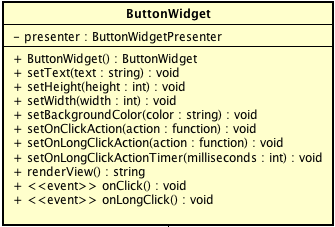
\includegraphics[scale=0.5]{Sezioni/SottosezioniST/img/ButtonWidget.png}
	\caption{monolith::component::widget::button::view::ButtonWidget}
\end{figure}

\begin{itemize}
\item \textbf{Descrizione}: Questa classe rappresenta un widget buttone, implementando l'interfaccia ButtonWidgetView.
\item \textbf{Utilizzo}: Implementando i metodi di ButtonWidgetView questa classe viene utilizzata al momento della creazione e della personalizzazione del bottone e delle sue reazioni alle azioni degli utenti.
\item \textbf{Attributi}: 
	\begin{itemize}
	\item \textit{private presenter:ButtonWidgetPresenter}\\
	Il presenter associato al widget bottone, al quale questa classe delega la gestione del comportamento del widget stesso.
	\end{itemize}
\item \textbf{Metodi}:
	\begin{itemize}
	\item \textit{ButtonWidget():ButtonWidget}\\
	Il costruttore della classe ButtonWidget.
	\item \textit{public renderView():string}\\
	 Genera il codice HTML CSS JS necessario per visualizzare il widget.
	\item \textit{public setText(text:string):void}\\
	Imposta il testo all'interno del bottone.
		\\ \textbf{Parametri}: \begin{itemize}
		\item \textit{text:string}\\
		Rappresenta il testo che verrà impostato all'interno del bottone.
		\end{itemize}
	\item \textit{public setHeight(height:int):void}\\
	Imposta l'altezza del bottone.
		\\ \textbf{Parametri}: \begin{itemize}
		\item \textit{height:int}\\
		Rappresenta il numero di pixel corrispondente all'altezza del bottone che verrà impostata.
		\end{itemize}
	\item \textit{public setWidth(width:int):void}\\
	Imposta la larghezza del bottone.
		\\ \textbf{Parametri}: \begin{itemize}
		\item \textit{width:int}\\
		Rappresenta il numero di pixel corrispondente alla larghezza del bottone che verrà impostata.
		\end{itemize}
	\item \textit{public setBackgroundColor(color:string):void}\\
	Imposta il colore di sfondo del bottone.
		\\ \textbf{Parametri}: \begin{itemize}
		\item \textit{color:string}\\
		Rappresenta la stringa in esadecimale corrispondente al colore che verrà impostata come sfondo del bottone.
		\end{itemize}
	\item \textit{public setOnClickAction(action:function):void}\\
	Questo metodo viene utilizzato per impostare l'azione che deve essere eseguita dopo il click normale del bottone.
		\\ \textbf{Parametri}: \begin{itemize}
		\item \textit{action:function}\\
		L'azione, sotto forma di funzione, che deve essere eseguita al click normale del bottone.
		\end{itemize}
	\item \textit{public setOnLongClickAction(action:function):void}\\
		Questo metodo viene utilizzato per impostare l'azione che deve essere eseguita dopo il click prolungato del bottone.
		\\ \textbf{Parametri}: \begin{itemize}
		\item \textit{action:function}\\
		L'azione, sotto forma di funzione, che deve essere eseguita al click prolungato del bottone.
		\end{itemize}
		\item \textit{public setOnLongClickActionTimer(milliseconds:int):void}\\
		Questo metodo viene utilizzato per impostare il timer per la pressione prolungata di un bottone.
				\\ \textbf{Parametri}: \begin{itemize}
				\item \textit{milliseconds:int}\\
				Tempo in millisecondi.
	\end{itemize}
	\end{itemize}
\item{Eventi}
	\begin{itemize}
	\item \textit{public onClick():void}\\
	Evento che rappresenta il click normale sul bottone, dopo il quale si può personalizzare la reazione del bottone.
	\item \textit{public onLongClick():void}\\
	Evento che rappresenta il click prolungato sul bottone, dopo il quale si può personalizzare la reazione del bottone.
	\end{itemize}
\end{itemize}

\subsubsection{monolith::component::widget::button::presenter::ButtonWidgetPresenter}

\label{monolith::component::widget::button::presenter::ButtonWidgetPresenter}
\begin{figure}[H]
	\centering
	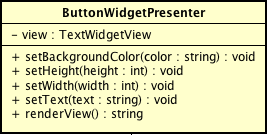
\includegraphics[scale=0.5]{Sezioni/SottosezioniST/img/ButtonWidgetPresenter.png}
	\caption{monolith::component::widget::button::presenter::ButtonWidgetPresenter}
\end{figure}

\begin{itemize}
\item \textbf{Descrizione}: Questa classe rappresenta il presenter per i widget di tipo bottone.
\item \textbf{Utilizzo}: Il presenter fa da tramite tra l'implementazione del widget e la view, formattando i dati che verranno visualizzati nella view e manipolando gli input dell'utente per eseguire le operazioni predisposte.
\item \textbf{Attributi}:
	\begin{itemize}
	\item \textit{private view:ButtonWidgetView}\\
	La view associata al presenter.
	\item \textit{private onClickAction:function}\\
	La funzione che il bottone eseguirà in seguito a un click normale.
	\item \textit{private onLongClicAction}\\
	La funzione che il bottone eseguirà in seguito a un click prolungato.
	\item \textit{private graphics:ButtonGraphics}\\
	L'oggetto che contiene le informazioni sullo stile visuale del bottone.
	\item \textit{private millisecondsBeforeOnLongClickActs:int}\\
	Tempo di pressione di un bottone in millisecondi dopo cui eseguire azioni in seguito ad un click prolungato.
	\end{itemize}
\item \textbf{Metodi}:
	\begin{itemize}
	\item \textit{ButtonWidgetPresenter(view:ButtonWidgetView):ButtonWidgetPresenter}\\
	Il costruttore della classe ButtonWidgetPresenter.
		\\ \textbf{Parametri}: \begin{itemize}
		\item \textit{view:ButtonWidgetView}\\
		La view necessaria alla costruzione del presenter.
		\end{itemize}
	\item \textit{public setOnClickAction(action:function):void}\\
	Questo metodo viene utilizzato per impostare l'azione che deve essere eseguita dopo il click normale del bottone.
		\\ \textbf{Parametri}: \begin{itemize}
		\item \textit{action:function}\\
		L'azione, sotto forma di funzione, che deve essere eseguita al click normale del bottone.
		\end{itemize}
	\item \textit{public setOnLongClickAction(action:function):void}\\
		Questo metodo viene utilizzato per impostare l'azione che deve essere eseguita dopo il click prolungato del bottone.
		\\ \textbf{Parametri}: \begin{itemize}
		\item \textit{action:function}\\
		L'azione, sotto forma di funzione, che deve essere eseguita al click prolungato del bottone.
		\end{itemize}
		\item \textit{public setOnLongClickActionTimer(milliseconds:int):void}\\
		Questo metodo viene utilizzato per impostare il timer per la pressione prolungata di un bottone.
				\\ \textbf{Parametri}: \begin{itemize}
				\item \textit{milliseconds:int}\\
				Tempo in millisecondi.
	\end{itemize}
	\item \textit{public setText(string text:int):void}\\
	Imposta il testo all'interno del bottone
		\\ \textbf{Parametri}: \begin{itemize}
		\item \textit{text:string}\\
		Rappresenta il testo che verrà impostato all'interno del bottone.
		\end{itemize}
	\item \textit{public setHeight(height:int):void}\\
	Imposta l'altezza del bottone.
		\\ \textbf{Parametri}: \begin{itemize}
		\item \textit{height:int}\\
		Rappresenta il numero di pixel corrispondente all'altezza del bottone che verrà impostata.
		\end{itemize}
	\item \textit{public setWidth(width:int):void}\\
	Imposta la larghezza del bottone.
		\\ \textbf{Parametri}: \begin{itemize}
		\item \textit{width:int}\\
		Rappresenta il numero di pixel corrispondente alla larghezza del bottone che verrà impostata.
		\end{itemize}
	\item \textit{public setBackgroundColor(color:string):void}\\
	Imposta il colore di sfondo del bottone.
		\\ \textbf{Parametri}: \begin{itemize}
		\item \textit{color:string}\\
		Rappresenta la stringa in esadecimale corrispondente al colore che verrà impostata come sfondo del bottone.
		\end{itemize}
	\item \textit{public renderView():string}\\
	Genera il codice HTML CSS JS necessario per visualizzare il widget.
	\end{itemize}
\end{itemize}

\subsubsection{monolith::component::widget::button::option::ButtonGraphics}

\label{monolith::component::widget::button::option::ButtonGraphics}
\begin{figure}[H]
	\centering
	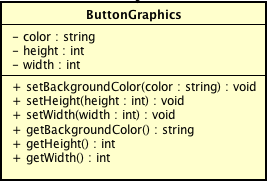
\includegraphics[scale=0.5]{Sezioni/SottosezioniST/img/ButtonGraphics.png}
	\caption{monolith::component::widget::button::option::ButtonGraphics}
\end{figure}

\begin{itemize}
\item \textbf{Descrizione}: Questa classe rappresenta l'aspetto visivo del bottone.
\item \textbf{Utilizzo}:
\item \textbf{Attributi}:
	\begin{itemize}
	\item \textit{private color:string}\\
	Rappresenta la stringa in esadecimale corrispondente al colore che verrà impostata come sfondo del bottone.
	\item \textit{private height:int}\\
	Rappresenta il numero di pixel corrispondente all'altezza del bottone. 
	\item \textit{private width:int}\\
	Rappresenta il numero di pixel corrispondente alla larghezza del bottone.
	\end{itemize}
\item \textbf{Metodi}:
	\begin{itemize}
	\item \textit{ButtonGraphics():ButtonGraphics}\\
	Il costruttore della classe ButtonGraphics.
	\item \textit{public setHeight(height:int):void}\\
	Imposta l'altezza del bottone.
		\\ \textbf{Parametri}: \begin{itemize}
		\item \textit{height:int}\\
		Rappresenta il numero di pixel corrispondente all'altezza del bottone che verrà impostata.
		\end{itemize}
	\item \textit{public setWidth(width:int):void}\\
	imposta la larghezza del bottone.
		\\ \textbf{Parametri}: \begin{itemize}
		\item \textit{width:int}\\
		Rappresenta il numero di pixel corrispondente alla larghezza del bottone che verrà impostata.
		\end{itemize}
	\item \textit{public setBackgroundColor(color:string):void}\\
	imposta il colore di sfondo del bottone.
		\\ \textbf{Parametri}: \begin{itemize}
		\item \textit{color:string}\\
		Rappresenta la stringa in esadecimale corrispondente al colore che verrà come sfondo del bottone.
		\end{itemize}
	\item \textit{public getHeight():int}\\
	Ritorna l'altezza del bottone.
	\item \textit{public getWidth():int}\\
	Ritorna la larghezza del bottone.
	\item \textit{public getBackgroundColor():string}\\
	Ritorna la stringa in esadecimale corrispondente al colore di sfondo del bottone.
	\end{itemize}
\end{itemize}

\subsubsection{monolith::component::widget::text::TextWidgetView}

\label{monolith::component::widget::text::TextWidgetView}
\begin{figure}[H]
	\centering
	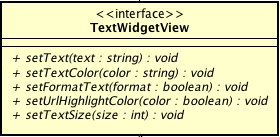
\includegraphics[scale=0.5]{Sezioni/SottosezioniST/img/TextWidgetView.png}
	\caption{monolith::component::widget::text::TextWidgetView}
\end{figure}

\begin{itemize}
\item \textbf{Descrizione}: Questa interfaccia rappresenta la view relativa ai widget di tipo testo.
\item \textbf{Utilizzo}: L'interfaccia viene utilizzata per disaccoppiare presenter e implementazione del widget e per visualizzare i dati che gli vengono passati dal presenter.
\item \textbf{Attributi}:
\item \textbf{Metodi}:
	\begin{itemize}
	\item \textit{public setText(text:string):void}\\
	Imposta il testo all'interno del widget testo.
		\\ \textbf{Parametri}: \begin{itemize}
		\item \textit{text:string}\\
		Rappresenta con una string il testo che va inserito all'interno del widget.
		\end{itemize}
	\item \textit{public setTextColor(color:string):void}\\
	Imposta il colore del testo del widget testo.
		\\ \textbf{Parametri}: \begin{itemize}
		\item \textit{color:string}\\
		Rappresenta la stringa in esadecimale corrispondente al colore che verrà come sfondo del bottone.
		\end{itemize}
	\item \textit{public setFormatText(format: boolean):void}\\
	Imposta il widget a testo formattato o testo semplice.
		\\ \textbf{Parametri}: \begin{itemize}
		\item \textit{format: boolean}\\
		Questo booleano viene impostato a true se si vuole il testo del widget formattato, a false altrimenti.
		\end{itemize} 
	\item \textit{public setUrlHighlightColor(color:boolean):void}\\
	Imposta la possibilità di cliccare o meno i link presenti nel testo del widget.
		\\ \textbf{Parametri}: \begin{itemize}
		\item \textit{color:string}\\
		Questo booleano viene impostato a true se si vogliono i link cliccabili, a false altrimenti.
		\end{itemize} 
	\item \textit{public setTextSize(size:int):void}\\
	Imposta la grandezza del testo nel widget
		\\ \textbf{Parametri}: \begin{itemize}
		\item \textit{size:int}\\
		Rappresenta il numero di pixel corrispondente all'altezza del testo che verrà impostata all'interno del widget.
		\end{itemize} 
	\end{itemize}
\end{itemize}

\subsubsection{monolith::component::widget::text::view::TextWidget}

\label{monolith::component::widget::text::view::TextWidget}
\begin{figure}[H]
	\centering
	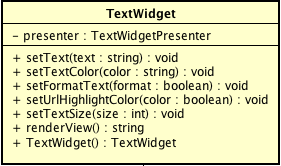
\includegraphics[scale=0.5]{Sezioni/SottosezioniST/img/TextWidget.png}
	\caption{monolith::component::widget::text::view::TextWidget}
\end{figure}

\begin{itemize}
\item \textbf{Descrizione}: Questa classe rappresenta un widget di testo, implementando l'interfaccia TextWidgetView
\item \textbf{Utilizzo}: Implementando i metodi di TextWidgetView questa classe viene utilizzata al momento della creazione e della personalizzazione del widget di testo e del suo contenuto.
\item \textbf{Attributi}:
	\begin{itemize}
	\item \textit{private presenter:TextWidgetPresenter}\\
	Il presenter associato al widget testo, al quale questa classe delega la gestione del comportamento del widget stesso.
	\end{itemize}
\item \textbf{Metodi}:
	\begin{itemize}
	\item \textit{public TextWidget():TextWidget}\\
	Il costruttore della classe TextWidget.
	\item \textit{public setText(text:string):void}\\
	Imposta il testo all'interno del widget testo.
		\\ \textbf{Parametri}: \begin{itemize}
		\item \textit{text:string}\\
		Rappresenta con una string il testo che va inserito all'interno del widget.
		\end{itemize} 
	\item \textit{public setTextColor(color:string):void}\\
	Imposta il colore del testo del widget testo.
		\\ \textbf{Parametri}: \begin{itemize}
		\item \textit{color:string}\\
		Rappresenta la stringa in esadecimale corrispondente al colore che verrà come sfondo del bottone.
		\end{itemize} 
	\item \textit{public setFormatText(format: boolean):void}\\
	Imposta il widget a testo formattato o testo semplice.
		\\ \textbf{Parametri}: \begin{itemize}
		\item \textit{format: boolean}\\
		Questo booleano viene impostato a true se si vuole il testo del widget formattato, a false altrimenti.
		\end{itemize} 
	\item \textit{public setUrlHighlightColor(color:boolean):void}\\
	Imposta la possiblità di cliccare o meno i link presenti nel testo del widget.
		\\ \textbf{Parametri}: \begin{itemize}
		\item \textit{color:string}\\
		Questo booleano viene impostato a true se si vogliono i link cliccabili, a false altrimenti.
		\end{itemize} 
	\item \textit{public setTextSize(size:int):void}\\
	Imposta la grandezza del testo nel widget
		\\ \textbf{Parametri}: \begin{itemize}
		\item \textit{size:int}\\
		Rappresenta il numero di pixel corrispondente all'altezza del testo che verrà impostata all'interno del widget.
		\end{itemize} 
	\item \textit{public renderView():string}\\
	Genera il codice HTML CSS JS necessario per visualizzare il widget.
	\end{itemize}
\end{itemize}

\subsubsection{monolith::component::widget::text::presenter::TextWidgetPresenter}

\label{monolith::component::widget::text::presenter::TextWidgetPresenter}
\begin{figure}[H]
	\centering
	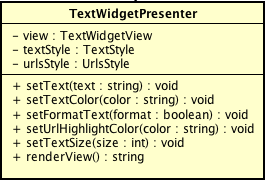
\includegraphics[scale=0.5]{Sezioni/SottosezioniST/img/TextWidgetPresenter.png}
	\caption{monolith::component::widget::text::presenter::TextWidgetPresenter}
\end{figure}

\begin{itemize}
\item \textbf{Descrizione}: Questa classe rappresenta il presenter per i widget di tipo testo.
\item \textbf{Utilizzo}: Il presenter fa da tramite tra l'implementazione del widget e la view,  formattando i dati che verranno visualizzati nella view.
\item \textbf{Attributi}:
	\begin{itemize}
	\item \textit{private view:TextWidgetView}\\
	La view associata al presenter.
	\item \textit{private textStyle:TextStyle}\\
	Stile del testo del widget.
	\item \textit{private urlsStyle:UrlsStyle}\\
	Stile dei link presenti all'interno del testo.
	\end{itemize}
\item \textbf{Metodi}:
	\begin{itemize}
	\item \textit{public TextWidgetPresenter(view:TextWidgetView):TextWidgetPresenter}\\
	Il costruttore della classe TextWidgetPresenter.
		\\ \textbf{Parametri}: \begin{itemize}
		\item \textit{view:TextWidgetView}\\
		La view necessaria alla costruzione del presenter.
		\end{itemize} 
	\item \textit{public setText(text:string):void}\\
	Imposta il testo all'interno del widget testo.
		\\ \textbf{Parametri}: \begin{itemize}
		\item \textit{text:string}\\
		Rappresenta con una string il testo che va inserito all'interno del widget.
		\end{itemize} 
	\item \textit{public setTextColor(color:string):void}\\
	Imposta il colore del testo del widget testo.
		\\ \textbf{Parametri}: \begin{itemize}
		\item \textit{color:string}\\
		Rappresenta la stringa in esadecimale corrispondente al colore che verrà impostato al testo all'interno del widget.
		\end{itemize} 
	\item \textit{public setFormatText(format: boolean):void}\\
	Imposta il widget a testo formattato o testo semplice.
		\\ \textbf{Parametri}: \begin{itemize}
		\item \textit{format: boolean}\\
		Questo booleano viene impostato a true se si vuole il testo del widget formattato, a false altrimenti.
		\end{itemize} 
	\item \textit{public setUrlHighlightColor(color:boolean):void}\\
	Imposta la possiblità di cliccare o meno i link presenti nel testo del widget.
		\\ \textbf{Parametri}: \begin{itemize}
		\item \textit{color:string}\\
		Questo booleano viene impostato a true se si vogliono i link cliccabili, a false altrimenti.
		\end{itemize} 
	\item \textit{public setTextSize(size:int):void}\\
	Imposta la grandezza del testo nel widget.
		\\ \textbf{Parametri}: \begin{itemize}
		\item \textit{size:int}\\
		Rappresenta il numero di pixel corrispondente all'altezza del testo che verrà impostata all'interno del widget.
		\end{itemize} 
	\item \textit{public renderView():string}\\
	Genera il codice HTML CSS JS necessario per visualizzare il widget.
	\end{itemize}
\end{itemize}

\subsubsection{monolith::component::widget::text::option::TextStyle}

\label{monolith::component::widget::text::option::TextStyle}
\begin{figure}[H]
	\centering
	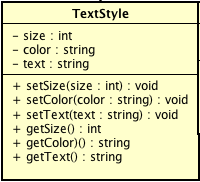
\includegraphics[scale=0.5]{Sezioni/SottosezioniST/img/TextStyle.png}
	\caption{monolith::component::widget::text::option::TextStyle}
\end{figure}

\begin{itemize}
\item \textbf{Descrizione}: Questa classe rappresenta lo stile del testo all'interno di un widget testo.
\item \textbf{Utilizzo}: La classe viene utilizzata ogniqualvolta vengono utilizzati metodi che cambiano lo stile visuale del testo in un widget testo.
\item \textbf{Attributi}:
	\begin{itemize}
	\item \textit{private size:int}\\
	Rappresenta il numero di pixel corrispondente all'altezza del testo.
	\item \textit{private color:string}\\
	Rappresenta la stringa in esadecimale corrispondente al colore del testo.
	\item \textit{private text:string}\\
	Rappresenta il testo stesso. 
	\item \textit{private formatted:boolean}\\
	Rappresenta l'impostazione del testo a formattato o meno.
	\end{itemize}
\item \textbf{Metodi}:
	\begin{itemize}
	\item \textit{public TextStyle():TextStyle}\\
	Il costruttore della classe TextStyle.
	\item \textit{public setSize(size:int):void}\\
	Imposta la grandezza del testo.
		\\ \textbf{Parametri}: \begin{itemize}
		\item \textit{size:int}\\
		Rappresenta il numero di pixel corrispondente all'altezza del testo che verrà impostata all'interno del widget.
		\end{itemize} 
	\item \textit{public setColor(color:string):void}\\
	Imposta il colore del testo del widget testo.
		\\ \textbf{Parametri}: \begin{itemize}
		\item \textit{color:string}\\
		Rappresenta la stringa in esadecimale corrispondente al colore che verrà impostato al testo all'interno del widget.
		\end{itemize} 
	\item \textit{public setText(string text:int):void}\\
	Imposta il testo.
		\\ \textbf{Parametri}: \begin{itemize}
		\item \textit{string text:int}\\
		Rappresenta con una string il testo che va inserito.
		\end{itemize} 
	\item \textit{public setFormatted(formatted:boolean):void}\\
	Imposta il testo a formattato o meno.
		\\ \textbf{Parametri}: \begin{itemize}
		\item \textit{formatted:boolean}\\
		Se questo booleano è a true il testo del widget viene formattato, se a false il testo viene considerato normale.
		\end{itemize} 
	\item \textit{public getSize():int}\\
	Ritorna il numero di pixel corrispondente all'altezza del testo.
	\item \textit{public getColor():string}\\
	Ritorna  la stringa in esadecimale corrispondente al colore del testo.
	\item \textit{public getText():string}\\
	Ritorna la stringa contenente il testo.
	\item \textit{public isFormatted():boolean}\\
	Ritorna true se il testo è formattato, false altrimenti.
	\end{itemize}
\end{itemize}

\subsubsection{monolith::component::widget::text::option::UrlStyle}

\label{monolith::component::widget::text::option::UrlsStyle}
\begin{figure}[H]
	\centering
	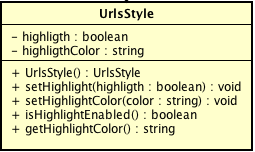
\includegraphics[scale=0.5]{Sezioni/SottosezioniST/img/UrlsStyle.png}
	\caption{monolith::component::widget::text::option::UrlsStyle}
\end{figure}

\begin{itemize}
\item \textbf{Descrizione}: Questa classe rappresenta lo stile del testo dei link all'interno di un widget testo.
\item \textbf{Utilizzo}: La classe viene utilizzata ogniqualvolta vengono utilizzati metodi che cambiano lo stile visuale dei link nel contenuto di un widget testo.
\item \textbf{Attributi}:
	\begin{itemize}
	\item \textit{private highlight:boolean}\\
	Booleano che rappresenta la possibilità o meno di cliccare i link nel testo.
	\item \textit{private highlightColor:string}\\
	Stringa in esadecimale corrispondente al colore dei link al testo all'interno del testo.
	\end{itemize}
\item \textbf{Metodi}:
	\begin{itemize}
	\item \textit{public UrlStyle():UrlsStyle}\\
	Il costruttore della classe UrlStyle.
	\item \textit{public setHighlight(color:boolean):void}\\
	Imposta la possiblità di cliccare o meno i link presenti nel testo.
		\\ \textbf{Parametri}: \begin{itemize}
		\item \textit{color:string}\\
		Questo booleano viene impostato a true se si vogliono i link cliccabili, a false altrimenti.
		\end{itemize} 
	\item \textit{public setHighlightColor(color:string):void}\\
	Imposta il colore del testo dei link presenti all'interno del testo.
		\\ \textbf{Parametri}: \begin{itemize}
		\item \textit{color:string}\\
		Rappresenta la stringa in esadecimale corrispondente al colore che verrà impostato per i link al testo all'interno del testo.
		\end{itemize} 
	\item \textit{public isHighlightEnabled():boolean}\\
	Ritorna true se i link sono cliccabili, false altrimenti.
	\item \textit{public getHighlightColor():string}\\
	Ritorna la stringa in esadecimale corrispondente al colore che verrà impostato per i link al testo all'interno del widget.
	\end{itemize}
\end{itemize}

\subsubsection{monolith::component::widget::checklist::ChecklistWidgetView}

\label{monolith::component::widget::checklist::ChecklistWidgetView}
\begin{figure}[H]
	\centering
	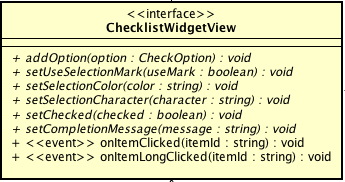
\includegraphics[scale=0.5]{Sezioni/SottosezioniST/img/ChecklistWidgetView.png}
	\caption{monolith::component::widget::checklist::ChecklistWidgetView}
\end{figure}

\begin{itemize}
\item \textbf{Descrizione}: Questa interfaccia rappresenta la view relativa ai widget di tipo checklist.
\item \textbf{Utilizzo}: L'interfaccia viene utilizzata per disaccoppiare presenter e implementazione del widget, visualizza i dati che gli vengono passati dal presenter.
\item \textbf{Attributi}:
\item \textbf{Metodi}:
	\begin{itemize}
	\item \textit{public addOption(option:CheckOption,onClick:function,onLongClick:function):void}\\
	Questo metodo aggiunge una opzione alla checklist.
		\\ \textbf{Parametri}: \begin{itemize}
		\item \textit{option:CheckOption}\\
		L'entry della checklist che verrà aggiunta.
		\item \textit{onClick:function}\\
		La funzione che viene eseguita al click normale di una entry della checklist.
		\item \textit{onLongClick:function}\\
		La funzione che viene eseguita al click prolungato di una entry della checklist.
		\end{itemize} 
	\item \textit{public setUseSelectionMark(useMark:boolean):void}\\
	Imposta la visualizzazione delle spunte con un carattere oppure con un colore.
		\\ \textbf{Parametri}: \begin{itemize}
		\item \textit{useMark:boolean}\\
		Se questo è a true la visualizzazione della spunta viene effettuata con un carattere, altrimenti la visualizzazione viene effettuata con un colore.
		\end{itemize}  
	\item \textit{public setSelectionColor(color:string):void}\\
	Imposta il colore con il quale effettuare la visualizzazione delle spunte.
		\\ \textbf{Parametri}: \begin{itemize}
		\item \textit{color:string}\\
		Rappresenta la stringa in esadecimale corrispondente al colore che verrà impostato per visualizzare le spunte.
		\end{itemize}  
	\item \textit{public setSelectionCharacter(character:string):void}\\
	Imposta il carattere utilizzato per la visualizzazione delle spunte.
		\\ \textbf{Parametri}: \begin{itemize}
		\item \textit{character:string}\\
		Il carattere utilizzato per la visualizzazione delle spunte.
		\end{itemize} 
	\item \textit{public setChecked(checked:boolean,position:int):void}\\
	Permette di spuntare un oggetto della checlist o di togliere una spunta da esso.
		\\ \textbf{Parametri}: \begin{itemize}
		\item \textit{checked:boolean}\\
		Questo booleano è a true se si vorrà spuntare la entry, a false altrimenti.
		\item \textit{position:int}\\
		La posizione, all'interno della checklist, dell'elemento del quale si vuole modificare lo stato. 
		\end{itemize}  
	\item \textit{public setCheckStyle(style:CheckStyle):void}\\
	Questo metodo imposta lo stile per le spunte delle opzioni della checklist.
		\\ \textbf{Parametri}: \begin{itemize}
		\item \textit{style:CheckStyle}\\
		Lo stile per le spunte delle opzioni della checklist che verrà impostata.
		\end{itemize}  
	\item \textit{public setCompletionMessage(message:string):void}\\
	Questo metodo imposta il messaggio di completamento che viene visualizzato quando tutte le opzioni della lista vengono spuntate.
		\\ \textbf{Parametri}: \begin{itemize}
		\item \textit{message:string}\\
		Stringa che rappresenta il messaggio di completamento della checklist.
		\end{itemize} 
	\item \textit{public emitOnListCompletedEvent():void}\\
	Questo metodo serve per lanciare l'evento di completamento della lista \texttt{onListCompleted()}.
	\end{itemize}
\item{Eventi}:
	\begin{itemize}
	\item \textit{public onItemClicked(itemId:string):void}\\
	Evento che rappresenta il click normale su una delle entry della lista, dopo il quale si può personalizzare la reazione della checklist.
		\\ \textbf{Parametri}: \begin{itemize}
		\item \textit{itemId:string}\\
		Id corrispondente all'entry della lista che è stata cliccata.
		\end{itemize} 
	\item \textit{public onItemLongClicked(itemId:string):void}\\
	Evento che rappresenta il click prolungato su una delle entry della lista, dopo il quale si può personalizzare la reazione della checklist.
		\\ \textbf{Parametri}: \begin{itemize}
		\item \textit{itemId:string}\\
		Id corrispondente all'entry della lista che è stata cliccata.
		\end{itemize} 
	\item \textit{public onListCompleted():void}\\
	Evento che rappresenta il completamento della checklist, ovvero quando tutte le sue entry sono spuntate.
	\end{itemize}
\end{itemize}

\subsubsection{monolith::component::widget::checklist::view::ChecklistWidget}

\label{monolith::component::widget::checklist::view::ChecklistWidget}
\begin{figure}[H]
	\centering
	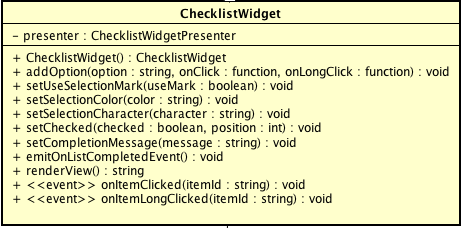
\includegraphics[scale=0.5]{Sezioni/SottosezioniST/img/ChecklistWidget.png}
	\caption{monolith::component::widget::checklist::view::ChecklistWidget}
\end{figure}

\begin{itemize}
\item \textbf{Descrizione}: Questa classe rappresenta un widget checklist, implementando l'interfaccia ChecklistWidgetView
\item \textbf{Utilizzo}: Implementando i metodi di ChecklistWidgetView questa classe viene utilizzata al momento della creazione e della personalizzazione del widget checklist e del suo contenuto.
\item \textbf{Attributi}:
	\begin{itemize}
	\item \textit{private presenter:ChecklistWidgetPresenter}\\
	Il presenter associato al widget checklist, al quale questa classe delega la gestione del comportamento del widget stesso.
	\end{itemize}
\item \textbf{Metodi}:
	\begin{itemize}
	\item \textit{public ChecklistWidget():ChecklistWidget}\\
	Il costruttore della classe ChecklistWidget.
	\item \textit{public addOption(option:CheckOption,onClick:function,onLongClick:function):void}\\
	Questo metodo aggiunge una entry alla checklist.
		\\ \textbf{Parametri}: \begin{itemize}
		\item \textit{option:CheckOption}\\
		L'entry della checklist che verrà aggiunta.
		\item \textit{onClick:function}\\
		La funzione che viene eseguita al click normale di una entry della checklist.
		\item \textit{onLongClick:function}\\
		La funzione che viene eseguita al click prolungato di una entry della checklist.
		\end{itemize} 
	\item \textit{public setUseSelectionMark(useMark:boolean):void}\\
		Imposta la visualizzazione delle spunte con un carattere oppure con un colore.
			\\ \textbf{Parametri}: \begin{itemize}
			\item \textit{useMark:boolean}\\
			Se questo è a true la visualizzazione della spunta viene effettuata con un carattere, altrimenti la visualizzazione viene effettuata con un colore.
			\end{itemize}  
	\item \textit{public setSelectionColor(color:string):void}\\
	Imposta il colore con il quale effettuare la visualizzazione delle spunte.
		\\ \textbf{Parametri}: \begin{itemize}
		\item \textit{color:string}\\
		Rappresenta la stringa in esadecimale corrispondente al colore che verrà impostato per visualizzare le spunte.
		\end{itemize}  
	\item \textit{public setSelectionCharacter(character:string):void}\\
	Imposta il carattere utilizzato per la visualizzazione delle spunte.
		\\ \textbf{Parametri}: \begin{itemize}
		\item \textit{character:string}\\
		Il carattere utilizzato per la visualizzazione delle spunte.
		\end{itemize}  
	\item \textit{public setChecked(checked:boolean,position:int):void}\\
	Permette di spuntare un oggetto della checlist o di togliere una spunta da esso.
		\\ \textbf{Parametri}: \begin{itemize}
		\item \textit{checked:boolean}\\
		Questo booleano è a true se si vorrà spuntare la entry, a false altrimenti.
		\item \textit{position:int}\\
		La posizione, all'interno della checklist, dell'elemento del quale si vuole modificare lo stato. 
		\end{itemize} 
	\item \textit{public setCheckStyle(style:CheckStyle):void}\\
	Questo metodo imposta lo stile per le spunte delle opzioni della checklist.
		\\ \textbf{Parametri}: \begin{itemize}
		\item \textit{style:CheckStyle}\\
		Lo stile per le spunte delle opzioni della checklist che verrà impostata.
		\end{itemize}  
	\item \textit{public setCompletionMessage(message:string):void}\\
	Questo metodo imposta il messaggio di completamento che viene visualizzato quando tutte le opzioni della lista vengono spuntate.
		\\ \textbf{Parametri}: \begin{itemize}
		\item \textit{message:string}\\
		Stringa che rappresenta il messaggio di completamento della checklist.
		\end{itemize} 
	\item \textit{public emitOnListCompletedEvent():void}\\
	Questo metodo serve per lanciare l'evento di completamento della lista \texttt{onListCompleted()}.
	\item \textit{public renderView():string}\\
	Genera il codice HTML CSS JS necessario per visualizzare il widget.
	\end{itemize}
\item{Eventi}:
	\begin{itemize}
	\item \textit{public onItemClicked(itemId:string):void}\\
	Evento che rappresenta il click normale su una delle entry della lista, dopo il quale si può personalizzare la reazione della checklist.
		\\ \textbf{Parametri}: \begin{itemize}
		\item \textit{itemId:string}\\
		Id corrispondente all'entry della lista che è stata cliccata.
		\end{itemize} 
	\item \textit{public onItemLongClicked(itemId:string):void}\\
	Evento che rappresenta il click prolungato su una delle entry della lista, dopo il quale si può personalizzare la reazione della checklist.
		\\ \textbf{Parametri}: \begin{itemize}
		\item \textit{itemId:string}\\
		Id corrispondente all'entry della lista che è stata cliccata.
		\end{itemize} 
	\end{itemize}
\end{itemize}

\subsubsection{monolith::component::widget::checklist::presenter::ChecklistWidgetPresenter}

\label{monolith::component::widget::checklist::presenter::ChecklistWidgetPresenter}
\begin{figure}[H]
	\centering
	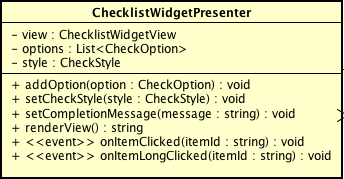
\includegraphics[scale=0.5]{Sezioni/SottosezioniST/img/ChecklistWidgetPresenter.png}
	\caption{monolith::component::widget::checklist::presenter::ChecklistWidgetPresenter}
\end{figure}

\begin{itemize}
\item \textbf{Descrizione}: Questa classe rappresenta il presenter per i widget di tipo checklist.
\item \textbf{Utilizzo}: Il presenter fa da tramite tra l'implementazione del widget e la view, formattando i dati che verranno visualizzati nella view e manipolando gli input dell'utente per eseguire le operazioni predisposte.
\item \textbf{Attributi}:
	\begin{itemize}
	\item \textit{private view:ChecklistWidgetView}\\
	La view associata al presenter.
	\item \textit{private options:List<CheckOption>}\\
	Collezione contentente tutte le opzioni della lista.
	\item \textit{private style:CheckStyle}\\
	Stile per le spunte della lista.
	\item \textit{private completionMessage:string}\\
	Stringa che contiene il messaggio di completamento della checklist.
	\end{itemize}
\item \textbf{Metodi}:
	\begin{itemize}
	\item \textit{public ChecklistWidgetPresenter(view:ChecklistWidgetView):ChecklistWidgetPresenter}\\
	Il costruttore della classe ChecklistWidgetPresenter.
		\\ \textbf{Parametri}: \begin{itemize}
		\item \textit{view:ChecklistWidgetView}\\
		La view necessaria alla costruzione del presenter.
		\end{itemize} 
	\item \textit{public addOption(option:CheckOption,onClick:function,onLongClick:function):void}\\
	Questo metodo aggiunge una entry alla checklist.
		\\ \textbf{Parametri}: \begin{itemize}
		\item \textit{option:CheckOption}\\
		L'entry della checklist che verrà aggiunta.
		\item \textit{onClick:function}\\
		La funzione che viene eseguita al click normale di una entry della checklist.
		\item \textit{onLongClick:function}\\
		La funzione che viene eseguita al click prolungato di una entry della checklist.
		\end{itemize} 
\item \textit{public setUseSelectionMark(useMark:boolean):void}\\
	Imposta la visualizzazione delle spunte con un carattere oppure con un colore.
		\\ \textbf{Parametri}: \begin{itemize}
		\item \textit{useMark:boolean}\\
		Se questo è a true la visualizzazione della spunta viene effettuata con un carattere, altrimenti la visualizzazione viene effettuata con un colore.
		\end{itemize}  
	\item \textit{public setSelectionColor(color:string):void}\\
	Imposta il colore con il quale effettuare la visualizzazione delle spunte.
		\\ \textbf{Parametri}: \begin{itemize}
		\item \textit{color:string}\\
		Rappresenta la stringa in esadecimale corrispondente al colore che verrà impostato per visualizzare le spunte.
		\end{itemize}  
	\item \textit{public setSelectionCharacter(character:string):void}\\
	Imposta il carattere utilizzato per la visualizzazione delle spunte.
		\\ \textbf{Parametri}: \begin{itemize}
		\item \textit{character:string}\\
		Il carattere utilizzato per la visualizzazione delle spunte.
		\end{itemize}   
	\item \textit{public setChecked(checked:boolean,position:int):void}\\
	Permette di spuntare un oggetto della checlist o di togliere una spunta da esso.
		\\ \textbf{Parametri}: \begin{itemize}
		\item \textit{checked:boolean}\\
		Questo booleano è a true se si vorrà spuntare la entry, a false altrimenti.
		\item \textit{position:int}\\
		La posizione, all'interno della checklist, dell'elemento del quale si vuole modificare lo stato. 
		\end{itemize}  
	\item \textit{public setCheckStyle(style:CheckStyle):void}\\
	Questo metodo imposta lo stile per le spunte delle opzioni della checklist.
		\\ \textbf{Parametri}: \begin{itemize}
		\item \textit{style:CheckStyle}\\
		Lo stile per le spunte delle opzioni della checklist che verrà impostata.
		\end{itemize} 
	\item \textit{public setCompletionMessage(message:string):void}\\
	Questo metodo imposta il messaggio di completamento che viene visualizzato quando tutte le opzioni della lista vengono spuntate.
		\\ \textbf{Parametri}: \begin{itemize}
		\item \textit{message:string}\\
		Stringa che rappresenta il messaggio di completamento della checklist.
		\end{itemize} 
	\item \textit{public renderView():string}\\
	Genera il codice HTML CSS JS necessario per visualizzare il widget.
	\end{itemize}
\item{Eventi}:
	\begin{itemize}
	\item \textit{public onItemClicked(itemId:string):void}\\
	Evento che rappresenta il click normale su una delle entry della lista, dopo il quale si può personalizzare la reazione della checklist.
		\\ \textbf{Parametri}: \begin{itemize}
		\item \textit{itemId:string}\\
		Id corrispondente all'entry della lista che è stata cliccata.
		\end{itemize} 
	\item \textit{public onItemLongClicked(itemId:string):void}\\
	Evento che rappresenta il click prolungato su una delle entry della lista, dopo il quale si può personalizzare la reazione della checklist.
		\\ \textbf{Parametri}: \begin{itemize}
		\item \textit{itemId:string}\\
		Id corrispondente all'entry della lista che è stata cliccata.
		\end{itemize} 
	\end{itemize}
\end{itemize}

\subsubsection{monolith::component::widget::checklist::option::CheckOption}

\label{monolith::component::widget::checklist::option::CheckOption}
\begin{figure}[H]
	\centering
	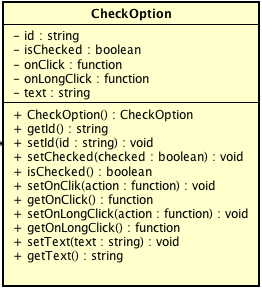
\includegraphics[scale=0.5]{Sezioni/SottosezioniST/img/CheckOption.png}
	\caption{monolith::component::widget::checklist::option::CheckOption}
\end{figure}

\begin{itemize}
\item \textbf{Descrizione}: La classe rappresenta una entry di un widget checklist.
\item \textbf{Utilizzo}: Viene utilizzata per ogni modifica di una checklist o evento relativo ad essa, poiché gli eventi della checklist sono relativi alle opzioni che ha al suo interno.
\item \textbf{Attributi}:
	\begin{itemize}
	\item \textit{private id:string}\\
	Stringa identificativa della entry della checklist.
	\item \textit{private isChecked:boolean}\\
	Booleano che rappresenta lo stato della entry, ovvero se questa è spuntata o no.
	\item \textit{private onClick:function}\\
	Funzione che verrà eseguita in seguito al click breve sulla entry.
	\item \textit{private onLongClick:function}\\
	Funzione che verrà eseguita in seguito al click prolungato sulla entry.
	\item \textit{private text:string}\\
	Questa stringa rappresenta il testo associato alla entry della checklist.
	\end{itemize}
\item \textbf{Metodi}:
	\begin{itemize}
	\item \textit{public CheckOption():CheckOption}\\
	Il costruttore della classe CheckOption.
	\item \textit{public getId():string}\\
	Ritorna l'id associato alla entry nella lista.
	\item \textit{public setId(id:string):void}\\
	Imposta l'id della entry con il valore passato.
		\\ \textbf{Parametri}: \begin{itemize}
		\item \textit{id:string}\\
			Valore da impostare come id della entry.
		\end{itemize}
	\item \textit{public getOnClick():string}\\
	Ritorna la funzione impostata come azione per il click normale della entry.
	\item \textit{public setOnClick(action:function):void}\\
	Imposta l'azione per il click normale della entry.
		\\ \textbf{Parametri}: \begin{itemize}
		\item \textit{action:function}\\
		La funzione che verrà impostata per il click normale della entry.
		\end{itemize} 
	\item \textit{public getOnLongClick():string}\\
	Ritorna la funzione impostata come azione per il click prolungato della entry.	
	\item \textit{public setOnLongClick(action:function):void}\\
	Imposta l'azione per il click prolungato della entry.	
		\\ \textbf{Parametri}: \begin{itemize}
		\item \textit{action:function}\\
		La funzione che verrà impostata per il click prolungato della entry.
		\end{itemize} 
	\item \textit{public setChecked(checked:boolean):void}\\
	Spunta la entry o toglie la spunta da essa.
		\\ \textbf{Parametri}: \begin{itemize}
		\item \textit{checked:boolean}\\
		Il metodo spunta la entry se questo campo è true, toglie la spunta se è false.
		\end{itemize} 
	\item \textit{public boolean isChecked()}\\
	Ritorna true se la entry è spuntata, false altrimenti.
	\item \textit{public getText():string}\\
	Ritorna la stringa contentente il testo associato alla entry della checklist.
	\item \textit{public setText(text:string):void}\\
	Imposta il testo associato alla entry della checklist.
		\\ \textbf{Parametri}: \begin{itemize}
		\item \textit{text:string}\\
		La stringa contentente il testo che verrà impostato come testo associato alla entry della checklist.
		\end{itemize} 
	\end{itemize}
\end{itemize}

\subsubsection{monolith::component::widget::checklist::option::CheckStyle}

\label{monolith::component::widget::checklist::option::CheckStyle}
\begin{figure}[H]
	\centering
	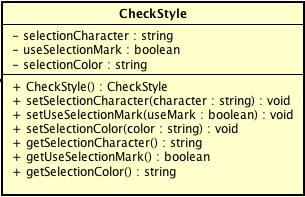
\includegraphics[scale=0.5]{Sezioni/SottosezioniST/img/CheckStyle.png}
	\caption{monolith::component::widget::checklist::option::CheckStyle}
\end{figure}

\begin{itemize}
\item \textbf{Descrizione}: La classe rappresenta lo stile con il quale vengono indicate le spunte su una entry di una checklist.
\item \textbf{Utilizzo}: Il suo utilizzo è legato alla scelta visuale dello sviluppatore per quanto riguarda lo stile con il quale viene evidenziata una selezione nella checklist.
\item \textbf{Attributi}:
	\begin{itemize}
	\item \textit{private selectionCharacter:string}\\
	Il carattere che viene utilizzato per la spunta delle entry della checklist.
	\item \textit{private useSelectionMark:boolean}\\
	Se questo booleano è a true, le spunte verranno visualizzate con un carattere, altrimenti verranno visualizzate evidenziando le entry con un colore.
	\item \textit{private selectionColor:string}\\
	Rappresenta la stringa in esadecimale corrispondente al colore che è impostato per evidenziare le opzioni spuntate della checklist.
	\end{itemize}
\item \textbf{Metodi}:
	\begin{itemize}
	\item \textit{public CheckStyle():CheckStyle}\\
	Il costruttore della classe CheckStyle.
	\item \textit{public setSelectionCharacter(character:string):void}\\
	Imposta il carattere per la spunta delle entry della checklist.
		\\ \textbf{Parametri}: \begin{itemize}
		\item \textit{character:string}\\
		Il carattere scelto per visualizzare le spunte.
		\end{itemize} 
	\item \textit{public setUseSelectionMark(useMark:boolean):void}\\
	Imposta l'utilizzo del carattere o del colore per evidenziare la spunta di una entry della checklist.
		\\ \textbf{Parametri}: \begin{itemize}
		\item \textit{useMark:boolean)}\\
		Se questo booleano è a true, le spunte verranno visualizzate con un carattere, altrimenti verranno visualizzate evidenziando le entry con un colore.
		\end{itemize} 
	\item \textit{public setSelectionColor(color:string):void}\\
	Imposta il colore per evidenziare le opzioni spuntate nella checklist.
		\\ \textbf{Parametri}: \begin{itemize}
		\item \textit{color:string}\\
		Rappresenta la stringa in esadecimale corrispondente al colore che verrà impostato per evidenziare le opzioni spuntate della checklist.
		\end{itemize} 
	\item \textit{public getSelectionCharacter():string}\\
	Ritorna il carattere che viene utilizzato per la spunta delle entry della checklist.
	\item \textit{public getUseSelectionMark():boolean}\\
	Ritorna true se viene utilizzato il carattere per visualizzare le spunte, altrimenti false.
	\item \textit{public getSelectionColor():string}\\
	Ritorna la stringa in esadecimale corrispondente al colore che è impostato per evidenziare le opzioni spuntate della checklist.
	\end{itemize}
\end{itemize}

\subsubsection{monolith::component::widget::list::ListWidgetView}

\label{monolith::component::widget::list::ListWidgetView}
\begin{figure}[H]
	\centering
	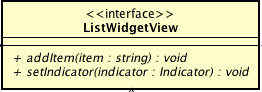
\includegraphics[scale=0.5]{Sezioni/SottosezioniST/img/ListWidgetView.png}
	\caption{monolith::component::widget::list::ListWidgetView}
\end{figure}

\begin{itemize}
\item \textbf{Descrizione}: Questa interfaccia rappresenta la view relativa ai widget di tipo lista.
\item \textbf{Utilizzo}: L'interfaccia viene utilizzata per disaccoppiare presenter e implementazione del widget, visualizza i dati che gli vengono passati dal presenter.
\item \textbf{Attributi}:
\item \textbf{Metodi}:
	\begin{itemize}
	\item \textit{public addItem(item:string):void}\\
	Aggiunge un oggetto alla lista.
		\\ \textbf{Parametri}: \begin{itemize}
		\item \textit{item:string}\\
		Il testo dell'oggetto da aggiungere alla lista.
		\end{itemize} 
	\item \textit{public setCharacter(character:string):void}\\
		Imposta il carattere utilizzato per indicare un elemento nella lista.
		\\ \textbf{Parametri}: \begin{itemize}
		\item \textit{character:string}\\
		Carattere da utilizzare per indicare un elemento nella lista.
		\end{itemize} 
	\item \textit{public setColor(color:string):void}\\
		Imposta il colore del carattere utilizzato per indicare un elemento nella lista.
		\\ \textbf{Parametri}: \begin{itemize}
		\item \textit{color:string}\\
		Codice esadecimale corrispondente al colore con il quale verrà colorato il carattere utilizzato per indicare un elemento nella lista.
		\end{itemize} 
	\end{itemize}
\end{itemize}

\subsubsection{monolith::component::widget::list::view::ListWidget}

\label{monolith::component::widget::list::view::ListWidget}
\begin{figure}[H]
	\centering
	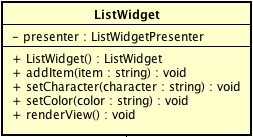
\includegraphics[scale=0.5]{Sezioni/SottosezioniST/img/ListWidget.png}
	\caption{monolith::component::widget::list::view::ListWidget}
\end{figure}

\begin{itemize}
\item \textbf{Descrizione}: Questa classe rappresenta un widget lista, un elenco di oggetti senza ordine, implementando l'interfaccia ListWidgetView.
\item \textbf{Utilizzo}: Implementando i metodi di ListWidgetView questa classe viene utilizzata al momento della creazione e della personalizzazione del widget lista e del suo contenuto.
\item \textbf{Attributi}:
	\begin{itemize}
	\item \textit{private presenter:ListWidgetPresenter}\\
	Il presenter associato al widget lista, al quale questa classe delega la gestione del comportamento del widget stesso.
	\end{itemize}
\item \textbf{Metodi}:
	\begin{itemize}
	\item \textit{public ListWidget():ListWidget}\\
	Il costruttore della class ListWidget.
	\item \textit{public addItem(item:string):void}\\
	Aggiunge un oggetto alla lista.
		\\ \textbf{Parametri}: \begin{itemize}
		\item \textit{item:string}\\
		Il testo dell'oggetto da aggiungere alla lista.
		\end{itemize} 
	\item \textit{public setCharacter(character:string):void}\\
	Imposta il simbolo che rappresenta l'indicatore dell'elenco puntato.
		\\ \textbf{Parametri}: \begin{itemize}
		\item \textit{character:string}\\
		La stringa contentente il simbolo che verrà impostato come indicatore dell'elenco puntato.
		\end{itemize} 
	\item \textit{public setColor(color:string):void}\\
	Imposta il colore dell'indicatore dell'elenco puntato.
		\\ \textbf{Parametri}: \begin{itemize}
		\item \textit{color:string}\\
		Rappresenta la stringa in esadecimale corrispondente al colore che verrà impostato per l'indicatore dell'elenco puntato.
		\end{itemize} 
	\item \textit{public renderView():string}\\
	Genera il codice HTML CSS JS necessario per visualizzare il widget.
	\end{itemize}
\end{itemize}

\subsubsection{monolith::component::widget::list::presenter::ListWidgetPresenter}

\label{monolith::component::widget::list::presenter::ListWidgetPresenter}
\begin{figure}[H]
	\centering
	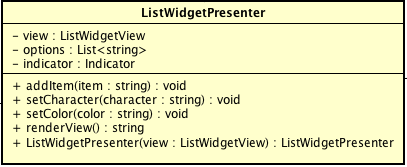
\includegraphics[scale=0.5]{Sezioni/SottosezioniST/img/ListWidgetPresenter.png}
	\caption{monolith::component::widget::list::presenter::ListWidgetPresenter}
\end{figure}

\begin{itemize}
\item \textbf{Descrizione}: Questa classe rappresenta il presenter per i widget di tipo lista.
\item \textbf{Utilizzo}: Il presenter fa da tramite tra l'implementazione del widget e la view, formattando i dati che verranno visualizzati nella view e manipolando gli input dell'utente per eseguire le operazioni predisposte.
\item \textbf{Attributi}:
	\begin{itemize}
	\item \textit{private view:ListWidgetView}\\
	La view associata al presenter.
	\item \textit{private options:List<string>}\\
	Questa collezione di stringhe rappresenta l'elenco di oggetti appartenenti alla lista.
	\item \textit{private indicator:Indicator}\\
	Il simbolo impostato per indicare gli oggetti della lista.
	\end{itemize}
\item \textbf{Metodi}:
	\begin{itemize}
	\item \textit{public ListWidgetPresenter(view:ListWidgetView):ListWidgetPresenter}\\
	Il costruttore della classe ListWidgetPresenter.
		\\ \textbf{Parametri}: \begin{itemize}
		\item \textit{view:ListWidgetView}\\
		La view necessaria alla costruzione del presenter.
		\end{itemize} 
	\item \textit{public addItem(item:string):void}\\
	Aggiunge un oggetto alla lista.
		\\ \textbf{Parametri}: \begin{itemize}
		\item \textit{item:string}\\
		Il testo dell'oggetto da aggiungere alla lista.
		\end{itemize} 
	\item \textit{public setCharacter(character:string):void}\\
	Imposta il simbolo che rappresenta l'indicatore dell'elenco puntato.
		\\ \textbf{Parametri}: \begin{itemize}
		\item \textit{character:string}\\
		La stringa contentente il simbolo che verrà impostato come indicatore dell'elenco puntato.
		\end{itemize} 
	\item \textit{public setColor(color:string):void}\\
	Imposta il colore dell'indicatore dell'elenco puntato.
		\\ \textbf{Parametri}: \begin{itemize}
		\item \textit{color:string}\\
		Rappresenta la stringa in esadecimale corrispondente al colore che verrà impostato per l'indicatore dell'elenco puntato.
		\end{itemize} 
	\item \textit{public renderView():string}\\
	Genera il codice HTML CSS JS necessario per visualizzare il widget.
	\end{itemize}
\end{itemize}

\subsubsection{monolith::component::widget::list::option::Indicator}

\label{monolith::component::widget::list::option::Indicator}
\begin{figure}[H]
	\centering
	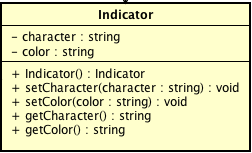
\includegraphics[scale=0.5]{Sezioni/SottosezioniST/img/Indicator.png}
	\caption{monolith::component::widget::list::option::Indicator}
\end{figure}

\begin{itemize}
\item \textbf{Descrizione}: Questa classe rappresenta l'indicatore per gli oggetti di un widget lista.
\item \textbf{Utilizzo}: Ogni lista ha un indicatore per i suoi oggetti, e questa classe fornisce gli strumenti per personalizzarlo.
\item \textbf{Attributi}:
	\begin{itemize}
	\item \textit{private character:string}\\
	Il simbolo impostato per indicare gli oggetti della lista.
	\item \textit{private color:string}\\
	Rappresenta la stringa in esadecimale corrispondente al colore che è impostato per gli indicatori.
	\end{itemize}
\item \textbf{Metodi}:
	\begin{itemize}
	\item \textit{public Indicator():Indicator}\\
	Il costruttore della classe Indicator.
	\item \textit{public setCharacter(character:string):void}\\
	Imposta il simbolo per indicare gli oggetti della lista.
		\\ \textbf{Parametri}: \begin{itemize}
		\item \textit{character:string}\\
		Il simbolo che verrà impostato per indicare gli oggetti della lista.
		\end{itemize} 
	\item \textit{public setColor(color:string):void}\\
	Imposta il colore degli indicatori.
		\\ \textbf{Parametri}: \begin{itemize}
		\item \textit{color:string}\\
		la stringa in esadecimale corrispondente al colore che verrà impostato per gli indicatori.
		\end{itemize} 
	\item \textit{public getCharacter():string}\\
	Ritorna il simbolo usato per indicare gli oggetti della lista.
	\item \textit{public getColor():string}\\
	Ritorna la stringa in esadecimale corrispondente al colore che è impostato per gli indicatori.
	\end{itemize}
\end{itemize}

\subsubsection{monolith::component::widget::image::ImageWidgetView}

\label{monolith::component::widget::image::ImageWidgetView}
\begin{figure}[H]
	\centering
	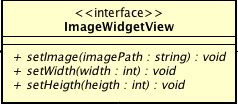
\includegraphics[scale=0.5]{Sezioni/SottosezioniST/img/ImageWidgetView.png}
	\caption{monolith::component::widget::image::ImageWidgetView}
\end{figure}

\begin{itemize}
\item \textbf{Descrizione}: Questa interfaccia rappresenta la view relativa ai widget di tipo immagine.
\item \textbf{Utilizzo}: L'interfaccia viene utilizzata per disaccoppiare presenter e implementazione del widget.
\item \textbf{Attributi}:
\item \textbf{Metodi}:
	\begin{itemize}
	\item \textit{public setImage(imagePath:string):void}\\
	Imposta il percorso nel file system che porta all'immagine che si vuole inserire nel widget.
		\\ \textbf{Parametri}: \begin{itemize}
		\item \textit{imagePath:string}\\
		Il percorso dell'immagine.
		\end{itemize} 
	\item \textit{public setHeight(height:int):void}\\
	Imposta l'altezza dell'immagine.
		\\ \textbf{Parametri}: \begin{itemize}
		\item \textit{height:int}\\
		L'altezza dell'immagine che si vuole impostare in pixel.
		\end{itemize} 
	\item \textit{public setWidth(width:int):void}\\
	Imposta la larghezza dell'immagine.
		\\ \textbf{Parametri}: \begin{itemize}
		\item \textit{width:int}\\
		La larghezza dell'immagine che si vuole impostare in pixel.
		\end{itemize} 
	\end{itemize}
\end{itemize}

\subsubsection{monolith::component::widget::image::view::ImageWidget}

\label{monolith::component::widget::image::view::ImageWidget}
\begin{figure}[H]
	\centering
	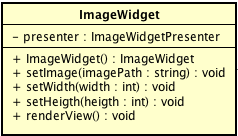
\includegraphics[scale=0.5]{Sezioni/SottosezioniST/img/ImageWidget.png}
	\caption{monolith::component::widget::image::view::ImageWidget}
\end{figure}

\begin{itemize}
\item \textbf{Descrizione}: Questa classe rappresenta un widget immagine, implementando l'interfaccia ImageWidgetView.
\item \textbf{Utilizzo}: Implementando i metodi di ImageWidgetView questa classe viene utilizzata al momento della creazione e della personalizzazione del widget immagine e del suo contenuto.
\item \textbf{Attributi}:
	\begin{itemize}
	\item \textit{private presenter:ImageWidgetPresenter}\\
	Il presenter associato al widget immagine, al quale questa classe delega la gestione del comportamento del widget stesso.
	\end{itemize}
\item \textbf{Metodi}:
	\begin{itemize}
	\item \textit{public ImageWidget():ImageWidget}\\
	Il costruttore della classe ImageWidget.
	\item \textit{public setImage(imagePath:string):void}\\
	Imposta il percorso nel file system che porta all'immagine che si vuole inserire nel widget.
		\\ \textbf{Parametri}: \begin{itemize}
		\item \textit{imagePath:string}: Il percorso dell'immagine.
		\end{itemize} 
	\item \textit{public setHeight(height:int):void}\\
	Imposta l'altezza dell'immagine.
		\\ \textbf{Parametri}: \begin{itemize}
		\item \textit{height:int}\\
		L'altezza dell'immagine che si vuole impostare in pixel.
		\end{itemize} 
	\item \textit{public setWidth(width:int):void}\\
	Imposta la larghezza dell'immagine.
		\\ \textbf{Parametri}: \begin{itemize}
		\item \textit{width:int}\\
		La larghezza dell'immagine che si vuole impostare in pixel.
		\end{itemize} 
	\item \textit{public renderView():string}\\
	Genera il codice HTML CSS JS necessario per visualizzare il widget.
	\end{itemize}
\end{itemize}

\subsubsection{monolith::component::widget::image::presenter::ImageWidgetPresenter}

\label{monolith::component::widget::image::presenter::ImageWidgetPresenter}
\begin{figure}[H]
	\centering
	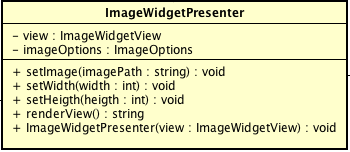
\includegraphics[scale=0.5]{Sezioni/SottosezioniST/img/ImageWidgetPresenter.png}
	\caption{monolith::component::widget::image::presenter::ImageWidgetPresenter}
\end{figure}

\begin{itemize}
\item \textbf{Descrizione}: Questa classe rappresenta il presenter per i widget di tipo lista.
\item \textbf{Utilizzo}: Il presenter fa da tramite tra l'implementazione del widget e la view, formattando i dati che verranno visualizzati nella view e manipolando gli input dell'utente per eseguire le operazioni predisposte.
\item \textbf{Attributi}:
	\begin{itemize}
	\item \textit{private view:ImageWidgetView}\\
	La view associata al presenter.
	\item \textit{private imageOptions:ImageOptions}\\
	Contiene le impostazioni attuali del widget.
	\end{itemize}
\item \textbf{Metodi}:
	\begin{itemize}
	\item \textit{public ImageWidgetPresenter(view:ImageWidgetView):ImageWidgetPresenter}\\
	Il costruttore della classe ImageWidgetPresenter.
		\\ \textbf{Parametri}: \begin{itemize}
		\item \textit{view:ImageWidgetView}\\
		La view necessaria alla costruzione del presenter.
		\end{itemize}
	\item \textit{public setImage(imagePath:string):void}\\
	Imposta il percorso nel file system che porta all'immagine che si vuole inserire nel widget.
		\\ \textbf{Parametri}: \begin{itemize}
		\item \textit{imagePath:string}\\
		Il percorso dell'immagine.
		\end{itemize} 
	\item \textit{public setHeight(height:int):void}\\
	Imposta l'altezza dell'immagine.
		\\ \textbf{Parametri}: \begin{itemize}
		\item \textit{height:int}\\
		L'altezza dell'immagine che si vuole impostare in pixel.
		\end{itemize} 
	\item \textit{public setWidth(width:int):void}\\
	Imposta la larghezza dell'immagine.
		\\ \textbf{Parametri}: \begin{itemize}
		\item \textit{width:int}\\
		La larghezza dell'immagine che si vuole impostare in pixel.
		\end{itemize} 
	\item \textit{public renderView():string}\\
	Genera il codice HTML CSS JS necessario per visualizzare il widget.
	\end{itemize}
\end{itemize}

\subsubsection{monolith::component::widget::image::option::ImageOptions}

\label{monolith::component::widget::image::option::ImageOptions}
\begin{figure}[H]
	\centering
	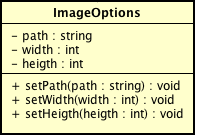
\includegraphics[scale=0.5]{Sezioni/SottosezioniST/img/ImageOptions.png}
	\caption{monolith::component::widget::image::option::ImageOptions}
\end{figure}

\begin{itemize}
\item \textbf{Descrizione}: Questa classe rappresenta le impostazioni di un widget immagine.
\item \textbf{Utilizzo}: Ogni cambiamento delle impostazioni di visualizzazione di un widget immagine coinvolge questa classe.
\item \textbf{Attributi}:
	\begin{itemize}
	\item \textit{private path:string}\\
	Il percorso dell'immagine.
	\item \textit{private width:int}\\
	L'altezza dell'immagine. 
	\item \textit{private height:int}\\
	La larghezza dell'immagine. 
	\end{itemize}
\item \textbf{Metodi}:
	\begin{itemize}
	\item \textit{public ImageOptions():ImageOptions}\\
	Il costruttore della classe ImageOptions.
	\item \textit{public setPath(path:string):void}\\
	Imposta il percorso nel file system che porta all'immagine che si vuole inserire nel widget.
		\\ \textbf{Parametri}: \begin{itemize}
		\item \textit{path:string}\\
		Il percorso dell'immagine.
		\end{itemize} 
	\item \textit{public setHeight(height:int):void}\\
	Imposta l'altezza dell'immagine.
		\\ \textbf{Parametri}: \begin{itemize}
		\item \textit{height:int}\\
		L'altezza dell'immagine che si vuole impostare  in pixel.
		\end{itemize} 
	\item \textit{public setWidth(width:int):void}\\
	Imposta la larghezza dell'immagine.
		\\ \textbf{Parametri}: \begin{itemize}
		\item \textit{width:int}\\
		La larghezza dell'immagine che si vuole impostare  in pixel.
		\end{itemize} 
	\end{itemize}
\end{itemize}